
\section{Resultados}

\subsection{Propiedades de la red y detección de comunidades}

En nuestra red vimos que todos los nodos estaban conectados entre sí y que se trataba de un grafo no dirigido.

\vspace{3pt}

Obtuvimos una tabla con el \textbf{grado de centralidad} de cada gen. Pudimos observar como el gen de interés TP53 es el que presentaba un mayor grado de centralidad y por tanto más relaciones con otros genes. 
\begin{figure}
	\centering
	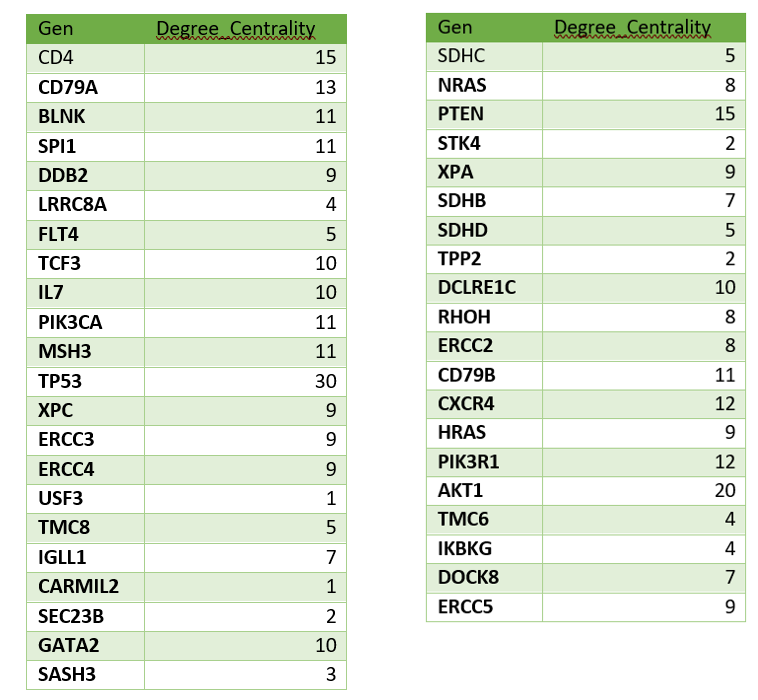
\includegraphics[width=0.8\linewidth]{grado_centralidad}
	\caption{Descripción de la figura.}
	\label{fig:grado_centralidad}
\end{figure}


\vspace{3pt}

En cuanto al \textbf{grado de conectividad} obtuvimos un valor del 19\%, el cual era bastante pequeño y nos indicaba que nuestro grafo no era muy fuerte. Esto puede deberse a que las comunidades entre si no tenían una gran dependencia y teníamos varios genes que no nos interesaban. 

\vspace{3pt}

Empleamos distintos algoritmos para \textbf{detectar comunidades}. En el caso del método de Girvan-Newman había nodos que no pertenecían a ninguna comunidad. Esto podía deberse a la forma en que el algoritmo de betweenness identifica comunidades. Puede detectar comunidades basándose en la centralidad de intermediación de los nodos, y algunos nodos pueden no estar claramente vinculados a una comunidad en función de esta medida.

\vspace{3pt}

Con el algoritmo voraz todos los nodos pertenecían a alguna comunidad. al igual que con el algoritmo de propagación de etiquetas. Sin embargo, en este último obtuvimos tan solo 3 comunidades por lo que la clusterización es mínima.  Con la aplicación del método de Louvain también resultaban menos comunidades que con el algoritmo voraz. Observamos 4 comunidades. 

\begin{figure}
	\centering
	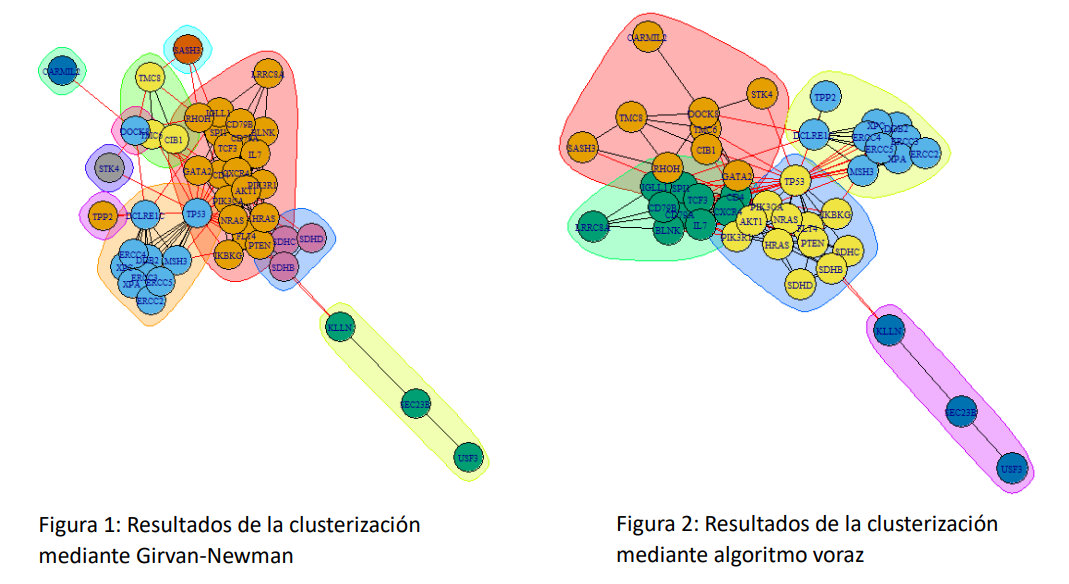
\includegraphics[width=0.8\linewidth]{cluster_GN_voraz}
	\caption{Descripción de la figura.}
	\label{fig:cluster_GN_voraz}
\end{figure} 

\begin{figure}
	\centering
	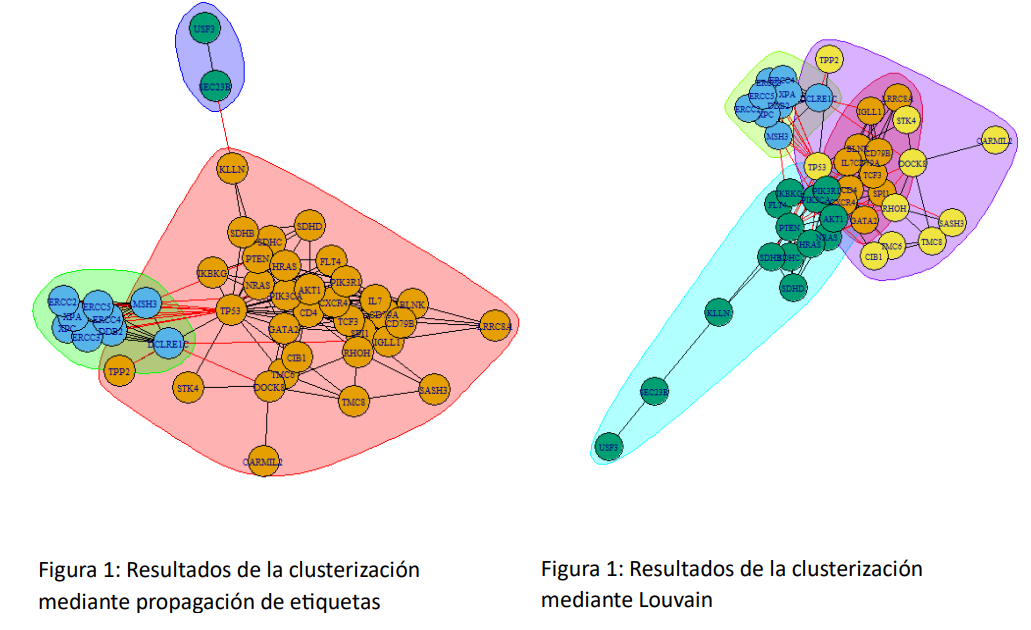
\includegraphics[width=0.8\linewidth]{cluster_etiq_louvain}
	\caption{Descripción de la figura.}
	\label{fig:cluster_etiq_louvain}
\end{figure}

Los algoritmos anteriores tenían la desventaja de que no reflejaban con exactitud la posibilidad de que un gen perteneciera a más de una comunidad. Para estudiar esto hicimos uso de \textbf{Link Communities}, y obtuvimos una gráfica donde cada gen era representado por un diagrama de sectores. Observamos que la mayoría de los genes pertenecen a más de una comunidad. Al centrarnos en nuestros genes de interés detectamos que el gen \textbf{TP53} tenía relación con 4 clusters distintos mientras que los otros genes de interés, SDHB, SDHb,HRAS, AKT1 se encontraban en una comunidad más diferenciada de color rosa. 

\begin{figure}
	\centering
	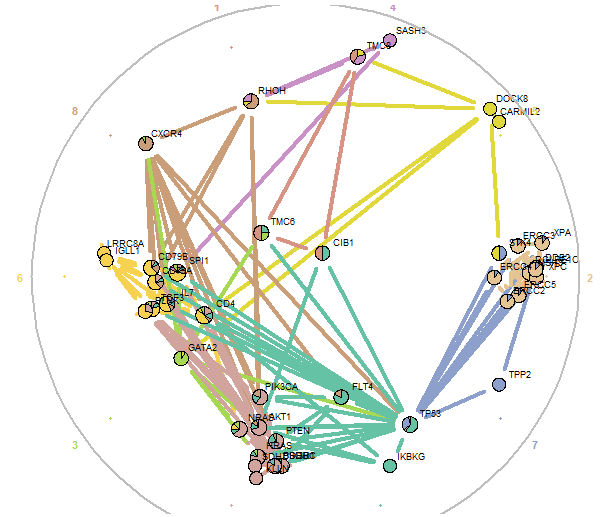
\includegraphics[width=0.8\linewidth]{link}
	\caption{Descripción de la figura.}
	\label{fig:link}
\end{figure}



Para el \textbf{estudio genes de interés} obtuvimos una tabla con dos columnas, el gen en concreto y sus genes vecinos. Observamos que todos los genes estaban relacionados entre sí menos el caso de TP53 y SDHD. 

\begin{figure}
	\centering
	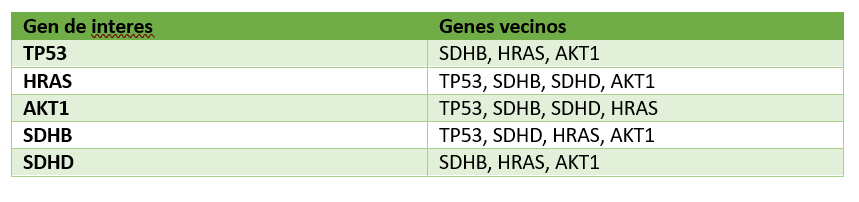
\includegraphics[width=0.8\linewidth]{gen_interes}
	\caption{Descripción de la figura.}
	\label{fig:gen_interes}
\end{figure}

